\documentclass[10pt]{beamer}

%packages
\usepackage{babel}
\usepackage[utf8]{inputenc}
\usepackage{amsmath,tabu}
\usepackage{color}
\usepackage{tikz}
\usepackage{pgfplots}
\usepackage{colortbl}
\usetikzlibrary{calc,shadings}
\usetikzlibrary{positioning}
\usepackage{eurosym}
\usepackage{mathtools}

%definitions
\usepackage{algorithm,algorithmic}

%theme
\usetheme{Dresden}
\usecolortheme{rose}
\useoutertheme{tree}

%environments
\newenvironment{ExampleGer}{\begin{exampleblock}{Beispiel}}{\end{exampleblock}}

\newenvironment{customlegend}[1][]{%
	\begingroup
	% inits/clears the lists (which might be populated from previous
	% axes):
	\csname pgfplots@init@cleared@structures\endcsname
	\pgfplotsset{#1}%
}{%
	% draws the legend:
	\csname pgfplots@createlegend\endcsname
	\endgroup
}%

%definitions
\def\addlegendimage{\csname pgfplots@addlegendimage\endcsname}
% definition to insert numbers
\pgfkeys{/pgfplots/number in legend/.style={%
		/pgfplots/legend image code/.code={%
			\node at (0.295,-0.0225){#1};
		},%
	},
}

%general
\title{A Deep Neural Network Approach to Splice Site Prediction}
\author{Tilman Hinnerichs}
\institute{Knowledge Mining Lab -- KAUST}
\date{\today}

%presentation
\expandafter\def\expandafter\insertshorttitle\expandafter{%
	\insertshorttitle\hspace{7cm}%
	\insertframenumber\,/\,\inserttotalframenumber
}
\begin{document}
	
\begin{frame}
	\titlepage
\end{frame}

\begin{frame}{Outline}
	\setbeamertemplate{section in toc}[sections numbered]
	\tableofcontents
\end{frame}

\section{Problem Description}
\begin{frame}{Problem Description}
	\begin{figure}[ht]
		\centering
		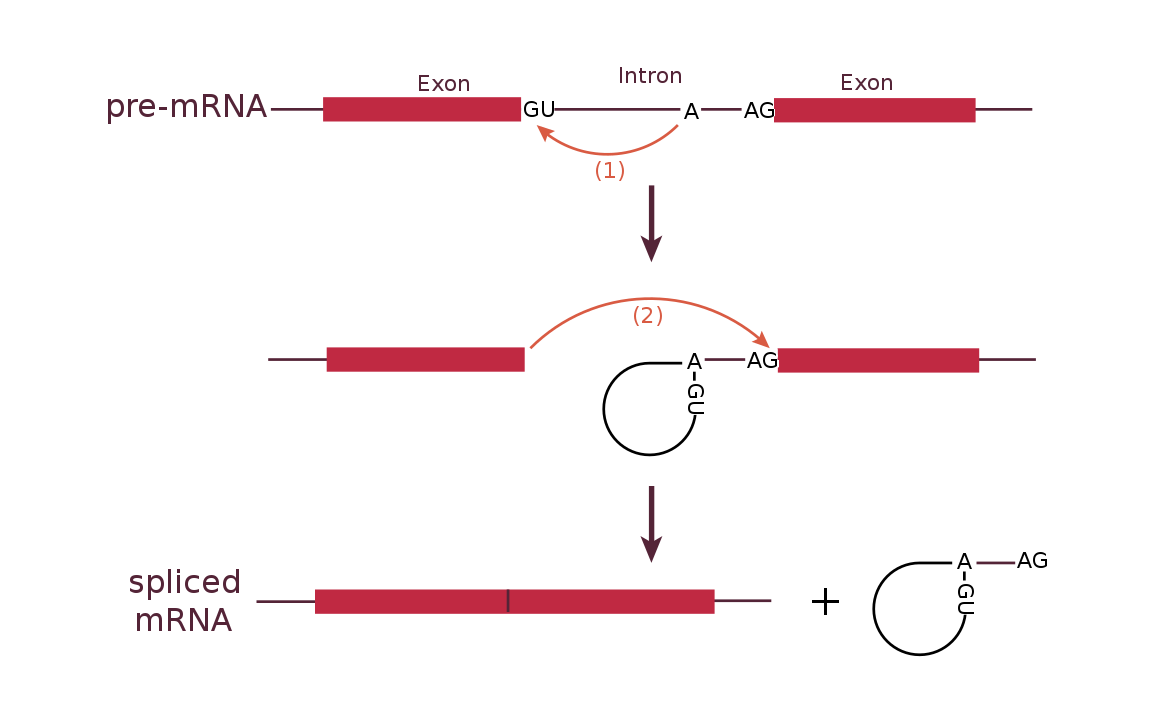
\includegraphics[width = 0.85\textwidth]{RNA_splicing_reaction.png}
		\caption{RNA splicing reaction (en.wikipedia.org)}
	\end{figure}
\end{frame}

\begin{frame}{Next Steps}
	\begin{itemize}
		\item Adapt convolution techniques from other papers with same goal
		\item Vary pre and post marker nt sequence length
		\item Use DiProDB[Friedel et al., NAR, 2009] for input
		\item Utilize electron io interaction potential (EIIP) for prediction
	\end{itemize}
\end{frame}

\end{document}